\chapter{パワー半導体デバイス ― 動作原理と選び方}
\label{chap3}

2章では，pn接合が「電圧の向きだけで電流を通したり止めたりする」ことを見た。
本章では，この物理を組み合わせて実際のパワー半導体素子を組み上げ，
その性能が材料と構造でどこまで決まるかを式で確かめ，最後に「どの素子をいつ選ぶか」まで下りる。
登場するダイオード・バイポーラトランジスタ（BJT）・MOSFET・IGBT・サイリスタの5つは，
どれもpn接合の並べ方と制御端子の付け方が違うだけで，
「いつオンにできるか」「どれだけ損失が出るか」がまったく変わる。

\begin{screen}
\noindent\textbf{この章の読み方}\\[3pt]
\begin{箇条書}
\item 各素子を\textbf{構造}→\textbf{なぜスイッチとして働くか}→\textbf{特徴}の順に読む。
道具は2章の空乏層とキャリアの注入だけである
\item \ref{sec3.7}節からは，耐圧・オン抵抗・スイッチング損失が互いに両立しないことを式で確かめ，
素子を選ぶ手順にまとめる
\end{箇条書}
\end{screen}

%%======================================================================
\section{スイッチに求められる3つの性能と，制御による分類}
\label{sec3.1}

\subsection{スイッチに求められる3つの性能}

エネルギーの流れ道を切り替えるスイッチ（序章）に求められる性能は，突き詰めると次の3つである。

\begin{箇条書}
\item \textbf{オフ状態}：高い電圧がかかっても電流を通さない（\textbf{耐圧}）
\item \textbf{オン状態}：大電流を小さい電圧降下で流す（低い\index{おんていこう@オン抵抗}\textbf{オン抵抗}）
\item \textbf{切り替え}：オンとオフを速く，小さい駆動電力で切り替えられる
\end{箇条書}

オン状態でオン抵抗$R_{\mathrm{on}}$に電流$I$が流れ続けることによる損失を
\index{どうつうそんしつ@導通損失}\textbf{導通損失}といい，
\begin{equation}
P_{\mathrm{on}} = R_{\mathrm{on}} I^2
\label{eq3.1}
\end{equation}
で表される。
また，切り替えの瞬間には素子に電圧と電流が同時にかかるため，切り替えのたびにエネルギーが失われる。
これを\index{すいっちんぐそんしつ@スイッチング損失}\textbf{スイッチング損失}という。
高い電圧に耐えるための低濃度の層は抵抗が大きい（2章）。
\textbf{耐圧を取ればオン抵抗が増える}というこのトレードオフに各素子がどう立ち向かうかが，本章の見どころである。

\subsection{制御のしかたによる分類}

実際の半導体スイッチには，制御端子の性質によって次の3段階がある。

\begin{箇条書}
\item \textbf{制御端子がない}：ダイオード。加わる電圧の向きだけでオン・オフが決まる
\item \textbf{オンだけ制御できる}：サイリスタ。オフは主回路の電流がゼロになるのを待つしかない
\item \textbf{オンもオフも制御できる}：BJT・MOSFET・IGBT
\end{箇条書}

\begin{定義}[自己消弧形と他励形]
\label{def3.1}
制御信号によって自らオフ（消弧）できる素子を\index{じこしょうこがた@自己消弧形}\textbf{自己消弧形}，
オフを外部回路の働き（電流が自然にゼロになること）に頼る素子を\index{たれいがた@他励形}\textbf{他励形}という。
BJT・MOSFET・IGBTは自己消弧形，サイリスタは他励形である。
\end{定義}

制御信号の与え方にも2通りある。
制御端子に\textbf{電流}を流し続けて主電流を制御する方式を
\index{でんりゅうくどう@電流駆動}\textbf{電流駆動}（BJT，サイリスタ），
制御端子に\textbf{電圧}をかけるだけで制御する方式を
\index{でんあつくどう@電圧駆動}\textbf{電圧駆動}（MOSFET，IGBT）という。
電流駆動はオンの間じゅう駆動電流を流し続ける電力が要る。
\FIGref{fig3.1}に5つの素子の記号と層構成，制御のしかたをまとめた。
用途でいえば，電鉄や直流送電のような大電力・低周波ではサイリスタ，電気自動車や産業用モータではIGBT，
電源装置や情報機器のような小容量・高周波ではMOSFETが主に使われる（\ref{sec3.9}節の\ref{fig3.9}）。

\begin{figure}[ht]
\begin{center}
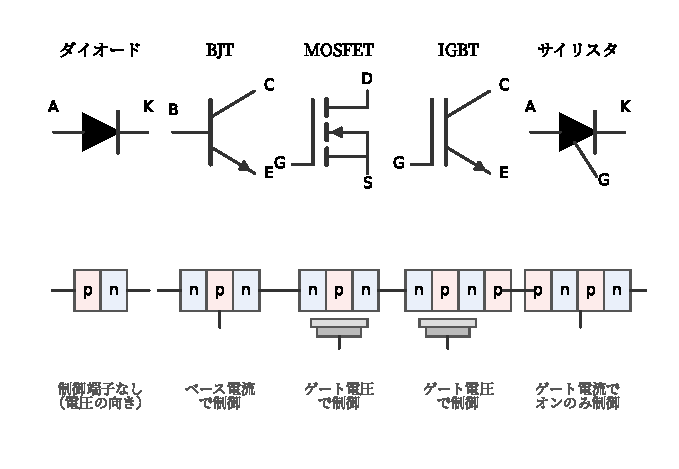
\includegraphics[clip]{figures/fig3.1.eps}
\end{center}
\caption{本章で扱う5つの半導体スイッチ。回路記号（上），半導体の層構成（下），
制御のしかた。どの素子もp形とn形の層の並べ方が違うだけである}
\label{fig3.1}
\end{figure}

%%======================================================================
\section{ダイオード ― 電圧の向きで切り替わる}
\label{sec3.2}

\subsection{構造 ― pn接合そのもの}

\index{だいおーど@ダイオード}\textbf{ダイオード}は，pn接合に電極を付けただけの最も簡単な素子である（\ref{fig3.1}）。
p形側の端子を\index{あのーど@アノード}\textbf{アノード}（A），n形側の端子を\index{かそーど@カソード}\textbf{カソード}（K）という。
接合面の空乏層には拡散電位$V_{bi}$（シリコンで約$0.7$\,V）の障壁がある。

\subsection{なぜスイッチとして働くか}

アノードを正にする順バイアス$v_D$をかけると障壁は$e(V_{bi}-v_D)$に下がり，障壁を越えて拡散するキャリアが急増する。
逆バイアスでは障壁が上がって電流はほとんど流れない。
障壁を越えられるキャリアの数は障壁の高さに対して指数関数的に変わるから，ダイオードの電流は
\begin{equation}
i_D = I_0 \left\{ \exp\left(\frac{e v_D}{kT}\right) - 1 \right\}
\label{eq3.2}
\end{equation}
と表される。
ここで$k$は\index{ぼるつまんていすう@ボルツマン定数}\textbf{ボルツマン定数}（$1.38\times10^{-23}$\,J/K），
$T$は絶対温度で，室温では$kT/e = 0.026$\,Vである。
$I_0$は\index{ぎゃくほうこうほうわでんりゅう@逆方向飽和電流}\textbf{逆方向飽和電流}と呼ばれるきわめて小さい電流である。

\FIGref{fig3.2}にダイオードの電流電圧特性を示す。
順方向では約$0.7$\,V付近から電流が急激に立ち上がり，「$0.7$\,Vでオンするスイッチ」として働く。
逆方向ではごく小さい漏れ電流しか流れないが，
逆電圧が\index{こうふくでんあつ@降伏電圧}\textbf{降伏電圧}$V_{BR}$に達すると，
空乏層内の電場が絶縁破壊電界（\ref{sec3.7}節）に達して電流が急増する（降伏）。

\begin{figure}[ht]
\begin{center}
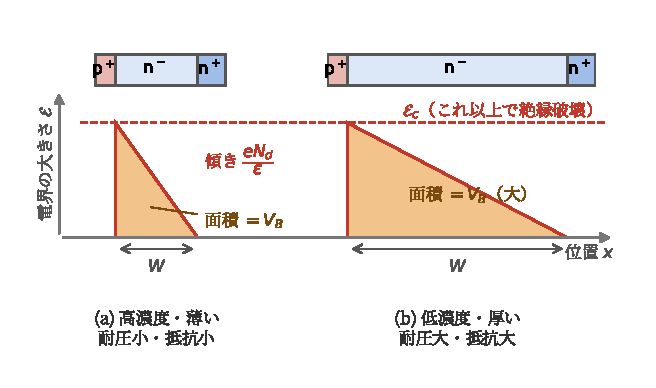
\includegraphics[clip]{figures/fig3.2.eps}
\end{center}
\caption{ダイオードの電流電圧特性。順方向は約0.7\,Vから立ち上がり，
逆方向は降伏電圧まで電流をほぼ遮断する}
\label{fig3.2}
\end{figure}

\subsection{特徴 ― 損失の質}

ダイオードの導通損失は，オン電圧がほぼ一定値$V_F \approx 0.7$\,Vに張り付くことから
\begin{equation}
P_{\mathrm{on}} = V_F I
\label{eq3.3}
\end{equation}
と電流の1乗で増え，$I^2$型の式\ref{eq3.1}とは損失の質が違う（章末問題\ref{ex3.3}）。
また，順方向に流れていたダイオードに急に逆電圧をかけると，
注入されていた少数キャリアが掃き出されるまでの短い時間，逆向きの電流が流れる。
これを\index{ぎゃくかいふく@逆回復}\textbf{逆回復}といい，スイッチング損失の原因になる（\ref{sec3.8}節）。
空乏層は正負の固定電荷が向かい合った平行平板キャパシタでもあり，
これを\index{せつごうようりょう@接合容量}\textbf{接合容量}という。その充放電もスイッチングの速さと損失を左右する。

%%======================================================================
\section{バイポーラトランジスタ ― 電流で制御する}
\label{sec3.3}

\index{ばいぽーらとらんじすた@バイポーラトランジスタ}\textbf{バイポーラトランジスタ}（BJT\index{BJT}）は，
n形・p形・n形の3層構造をもつ素子で（\ref{fig3.1}），
端子を\index{えみった@エミッタ}\textbf{エミッタ}（E），\index{べーす@ベース}\textbf{ベース}（B），
\index{これくた@コレクタ}\textbf{コレクタ}（C）という。
エミッタは高濃度にドーピングされ，中央のベースは\textbf{薄く}（数〜数十$\mathrm{\mu m}$）かつ\textbf{低濃度}に作られている。
エミッタとベースの間を順バイアス，ベースとコレクタの間を逆バイアスにすると，キャリアは次の3段階で動く。

\begin{箇条書}
\item \textbf{注入}：順バイアスで障壁が下がり，高濃度のエミッタから大量の電子がベースへ流れ込む
\item \textbf{拡散}：電子はベースの少数キャリアとなってコレクタ側へ拡散する。
ベースが薄いので，大部分（99\,\%程度）は正孔と再結合する前に通り抜ける
\item \textbf{回収}：逆バイアスのベースとコレクタの接合の強い電場が，たどり着いた電子をコレクタへ引き込む
\end{箇条書}

電子がベースを渡り切る時間は再結合の寿命の100分の1ほどしかないので，再結合で失われるのは1\,\%程度にとどまる。
それでもベースの正孔は再結合とエミッタへの逆向きの注入とで少しずつ失われ，正孔が減ると順バイアスが保てなくなって注入が止まる。
\textbf{ベース電流は，失われる正孔を外から補充し続けるための電流}であり，補充を止めれば（$i_B = 0$）素子はオフする。
$i_E = i_C + i_B$のうち，電子の99\,\%がコレクタへ抜けるならコレクタ電流はベース電流の99倍になる。この比
\begin{equation}
\beta = \frac{i_C}{i_B}
\label{eq3.4}
\end{equation}
を\index{でんりゅうぞうふくりつ@電流増幅率}\textbf{電流増幅率}といい，実際の素子では数十〜数百である。
$i_C = \beta i_B$が成り立つ状態を\index{かっせいりょういき@活性領域}\textbf{活性領域}という。
オフ（遮断）とフルオン（飽和）の\textbf{あいだ}でコレクタ電流が連続的に変わる領域で，
ここにとどめて使えば電圧を滑らかに調整できる（リニアレギュレータ，7章）。

BJTは電流駆動の自己消弧形スイッチである。
たとえば$\beta = 50$の素子で$100$\,Aを流すにはベース電流$2$\,Aが要り，
ベースとエミッタの間の電圧を$0.7$\,Vとすれば駆動電力は$1.4$\,Wにもなる。
オンの間じゅうこの電流を供給し続ける駆動回路が要るため，パワー用途の主役の座は電圧駆動のMOSFETとIGBTに譲られた。
それでも「pn接合の障壁をキャリア注入で開け閉めする」というBJTの動作は，以降のIGBTとサイリスタの部品になる。

%%======================================================================
\section{MOSFET ― 電圧で通り道を作る}
\label{sec3.4}

\subsection{構造 ― 絶縁されたゲート}

\index{MOSFET}\textbf{MOSFET}（metal-oxide-semiconductor field-effect transistor）の構造を\FIGref{fig3.3}(a)に示す。
p形の半導体に2つのn形領域を作り，それぞれ
\index{そーす@ソース}\textbf{ソース}（S）と\index{どれいん@ドレイン}\textbf{ドレイン}（D）の電極を付ける。
2つのn形領域にはさまれたp形表面の上に，薄い\index{さんかまく@酸化膜}\textbf{酸化膜}（絶縁体）を介して
\index{げーと@ゲート}\textbf{ゲート}（G）電極を置く。
ゲートは絶縁体の上に載っているから，\textbf{ゲートに直流電流は流れない}。
ゲート電圧がゼロなら，向かい合った2つのpn接合の一方が必ず逆バイアスになるので電流は流れない（オフ状態）。

\begin{figure}[ht]
\begin{center}
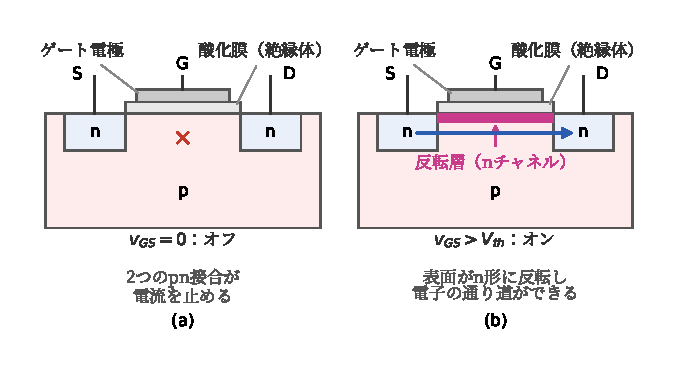
\includegraphics[clip]{figures/fig3.3.eps}
\end{center}
\caption{MOSFETの構造と反転層。(a)ゲート電圧がなければ2つのpn接合が電流を止める。
(b)ゲートに正電圧をかけると酸化膜の下のp形表面がn形に反転し，
ソースとドレインをつなぐ電子の通り道（nチャネル）ができる}
\label{fig3.3}
\end{figure}

\subsection{なぜスイッチとして働くか ― 電場が反転層を作る}

ゲートに正電圧$v_{GS}$をかけると，酸化膜をはさんだキャパシタの電場でp形表面の正孔は押しのけられ，電子が引き寄せられる。
電圧を上げていくと表面では電子の濃度が正孔の濃度を追い越し，p形だった表面がごく薄い層だけn形に「反転」する。

\begin{定義}[反転層としきい値電圧]
\label{def3.2}
ゲート電圧によって半導体表面にできる，もとの導電形と逆の形の薄いキャリア層を
\index{はんてんそう@反転層}\textbf{反転層}という。
n形の反転層はソースとドレインをつなぐ電子の通り道となるのでn\index{ちゃねる@チャネル}\textbf{チャネル}とも呼ぶ。
反転層ができ始めるゲート電圧を\index{しきいちでんあつ@しきい値電圧}\textbf{しきい値電圧}$V_{th}$という
（パワーMOSFETで2〜4\,V程度）。
\end{定義}

$v_{GS} > V_{th}$になると反転層を通ってソースからドレインへ電子が流れ（\ref{fig3.3}(b)），ゲート電圧を切れば反転層は消えて電流は止まる。
\textbf{電場でキャリアの通り道そのものを作ったり消したりする} ― これが電界効果トランジスタという名前の意味である。

\subsection{特徴 ― 下駄のない抵抗として振る舞う}

\FIGref{fig3.4}にMOSFETの出力特性を示す。特性が\textbf{原点からまっすぐ立ち上がる}。
電子はソース→反転層→ドレインとすべてn形の中を\textbf{一度もpn接合の障壁を越えずに}流れるから，
0.7\,Vのようなオン電圧の下駄がない。
オン状態のMOSFETは単なる抵抗$R_{\mathrm{on}}$として振る舞い，導通損失は式\ref{eq3.1}の型になる。
多数キャリアの電子だけで動くので少数キャリアの蓄積がなく，オフへの切り替えも速い。
ゲートは絶縁されているから定常状態では電流が流れず\textbf{駆動電力はほぼゼロ}で，
スイッチングの瞬間だけ，ゲートと半導体がなすキャパシタ（\index{げーとようりょう@ゲート容量}\textbf{ゲート容量}）を
充放電する電流が流れる。

\begin{figure}[ht]
\begin{center}
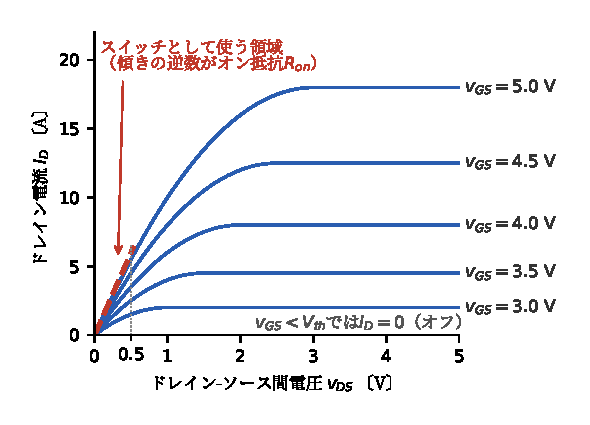
\includegraphics[clip]{figures/fig3.4.eps}
\end{center}
\caption{MOSFETの出力特性。原点から直線的に立ち上がる（オン電圧の下駄がない）ので，
オン状態は抵抗$R_{\mathrm{on}}$とみなせる。
原点付近の直線の傾きの逆数$v_{DS}/i_D$が$R_{\mathrm{on}}$で，$v_{GS}$が高いほど反転層の電子が多く$R_{\mathrm{on}}$は小さい}
\label{fig3.4}
\end{figure}

\begin{注意}
\ref{fig3.4}の原点付近の直線部分を\index{せんけいりょういき@線形領域}\textbf{線形領域}，
電流が$v_{DS}$によらずほぼ一定になる右側の部分を\index{ほうわりょういき@飽和領域}\textbf{飽和領域}と呼ぶ。
MOSFETの「飽和領域」はBJTの活性領域に相当し（7章のリニアレギュレータで使う），
BJTの「飽和」（フルオン）とは意味が入れ違っている。スイッチとして使うのは線形領域である。
\end{注意}

\ref{fig3.3}のように電流がチップの表面を横に流れる\index{よこがた@横型}\textbf{横型}は，電流の通る断面が薄く大電流には向かない。
そこでパワーMOSFETでは，\FIGref{fig3.5}(a)のようにドレインを裏面に置いて電流を表から裏へ縦に流す
\index{たてがた@縦型}\textbf{縦型}構造を使い，チップの全面を通り道にしてオン抵抗を下げる。
耐圧を受け持つ低濃度のn$^-$層を\index{どりふとそう@ドリフト層}\textbf{ドリフト層}といい，
その厚さと濃度で耐圧を設計する（\ref{sec3.7}節）。

\begin{figure}[ht]
\begin{center}
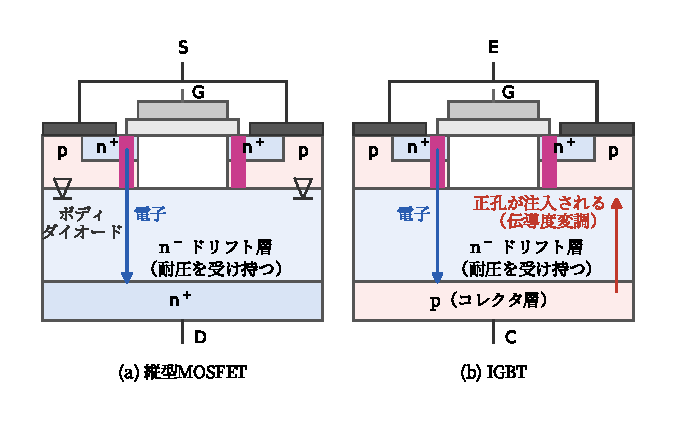
\includegraphics[clip]{figures/fig3.5.eps}
\end{center}
\caption{縦型パワーMOSFETとIGBTの断面。(a)縦型MOSFETは電流を表から裏へ縦に流し，
n$^-$ドリフト層が耐圧を受け持つ。(b)IGBTは裏面にp形層を加えた4層構造。
オン時にこの層から正孔が注入され，ドリフト層の抵抗が下がる（伝導度変調）}
\label{fig3.5}
\end{figure}

縦型では，ソース電極がn$^+$領域とそれを囲むp形の\index{ぼでぃ@ボディ}\textbf{ボディ}の両方に接しているため，
ボディとドリフト層の間のpn接合が\index{ぼでぃだいおーど@ボディダイオード}\textbf{ボディダイオード}として残り，
ソースを正にするとゲート電圧によらず電流が流れる。
つまり縦型MOSFETは\textbf{逆方向には常に導通する}素子で，インバータで還流ダイオードを省ける利点（9章）になる一方，逆回復を伴う。
ただし耐圧を上げようとドリフト層を厚く・低濃度にするとその抵抗が増え，
シリコンのMOSFETが得意なのはおおむね数百V以下である。それ以上を受け持つのが次のIGBTである。

\begin{問}
\item (a) \ref{fig3.4}の$v_{GS} = 5$\,Vの曲線は，原点付近では$v_{DS} = 0.5$\,Vのとき$i_D \approx 6$\,Aを通る直線とみなせる。
このときのオン抵抗$R_{\mathrm{on}}$を求めよ。
(b) MOSFETの駆動電力が定常状態でほぼゼロである理由と，それでもスイッチングの瞬間にはゲート電流が流れる理由を説明せよ。
\end{問}

%%======================================================================
\section{IGBT ― 伝導度変調で低損失}
\label{sec3.5}

\subsection{構造 ― 縦型MOSFETにp形層を1枚加える}

\index{IGBT}\textbf{IGBT}（insulated gate bipolar transistor）の構造を\ref{fig3.5}(b)に示す。
縦型MOSFETの裏面のn$^+$層を\textbf{p形の層に置き換えた}だけで，全体はn，p，n$^-$，pの4層構造になる。
端子は\textbf{エミッタ}（E），\textbf{ゲート}（G），\textbf{コレクタ}（C）と呼ぶ。

\subsection{なぜ低損失か ― 電子の川に正孔を注ぎ込む}

ゲートの働きはMOSFETと同じで，$v_{GS} > V_{th}$で反転層ができ，エミッタのn$^+$領域から電子がn$^-$ドリフト層へ流れ込む。
流れ込んだ電子がドリフト層にたまると，裏面のn$^-$層とp層の接合が\textbf{順バイアス}になり，
p形コレクタ層から大量の\textbf{正孔}がドリフト層へ注入される。
このように低濃度の層に電子と正孔が注入されて，キャリア濃度がドーピング濃度よりけた違いに増え，
抵抗が大幅に下がる現象を\index{でんどうどへんちょう@伝導度変調}\textbf{伝導度変調}という。
導電率$\sigma = e(n\mu_n + p\mu_p)$はキャリア濃度に比例するから（2章），
$10^{14}\,\mathrm{cm^{-3}}$程度のドリフト層でも，注入でキャリアが$10^{16}\,\mathrm{cm^{-3}}$以上に増えれば抵抗は100分の1以下になる。
\textbf{オフのときは低濃度層として高い電圧に耐え，オンのときはキャリア注入で低抵抗に化ける} ―
IGBTは，耐圧とオン抵抗のトレードオフをキャリア注入で骨抜きにする素子である。

\subsection{特徴 ― 得たものと引き換えにしたもの}

IGBTは電圧駆動と低損失を併せもち，600\,V以上・数十A以上の中〜大容量領域の主役である。
ただし代償が2つある。
第一に，主電流が裏面のpn接合を1つ通るため，オン電圧に約$0.7$\,Vの下駄が乗る
（導通損失は式\ref{eq3.3}の$V_{\mathrm{on}}I$型に近い）。
第二に，ターンオフのときにドリフト層にたまった大量の少数キャリアが消えるまで電流が流れ続ける。
この尾を引く電流を\index{てーるでんりゅう@テール電流}\textbf{テール電流}といい，
スイッチング損失を増やすため，IGBTの動作周波数はMOSFETより低め（数k〜数十kHz）にとどまる。

\begin{問}
\item IGBTのオン電圧には，MOSFETにはない約$0.7$\,Vの下駄が乗る。その理由を構造（\ref{fig3.5}(b)）に基づいて説明せよ。
\end{問}

%%======================================================================
\section{サイリスタ ― ラッチするスイッチ}
\label{sec3.6}

\index{さいりすた@サイリスタ}\textbf{サイリスタ}はp，n，p，nの4層構造をもつ素子で，
両端の端子を\textbf{アノード}（A）と\textbf{カソード}（K），内側のp層に付けた制御端子を\textbf{ゲート}（G）という（\ref{fig3.1}）。
IGBTと同じ4層だが，ゲートが酸化膜の上ではなく\textbf{p層に直接}つながっており，制御はゲート\textbf{電流}で行う。

アノードを正にしても，中央の接合が逆バイアスとなって電圧を支えるので，すぐにはオンしない。
4層構造は上半分のnpnトランジスタと下半分のpnpトランジスタが中央の2層を共有した形とみなせ，
ゲート電流でnpnがオンすると，そのコレクタ電流がpnpのベース電流になってpnpもオンし，
pnpのコレクタ電流がnpnのベースへ戻る ― \textbf{2つのトランジスタが互いにベース電流を供給し合う}。
この正のループが一巡すると外からのゲート電流は不要になり，全層が伝導度変調の起きた導通状態に入る。
いったんオンしたサイリスタは\textbf{ゲート電流を切ってもオンし続ける}。
この性質を\index{らっちどうさ@ラッチ動作}\textbf{ラッチ動作}という。
オフにするには，主回路の電流を外部回路の働きで
\index{ほじでんりゅう@保持電流}\textbf{保持電流}（ループが回り続けるのに必要な最小の主電流）以下まで減らすしかない。
これが他励形と呼ばれる理由である。

自分でオフできないことは，交流回路ではむしろ好都合である。
交流電流は半周期ごとに必ずゼロを通るから，オフはその自然なゼロ点に任せ，オンのタイミングだけをゲートで選べばよい（8章の位相制御整流）。
サイリスタは構造が単純で数kV・数kAの大電力を扱えるが，オフを商用周波数のゼロ点に頼るため高速スイッチングはできない。
なお，IGBTの内部にも同じ4層の寄生サイリスタが潜んでおり，定格を超える大電流でこれがラッチするとゲートで止められなくなる（ラッチアップ）。
意図してラッチさせるのがサイリスタ，ラッチしないよう設計するのがIGBTである。

%%======================================================================
\section{耐圧とオン抵抗のトレードオフ}
\label{sec3.7}

\subsection{耐圧 ― 空乏層が電圧を受け持つ}

逆バイアスの電圧はほぼすべて空乏層が受け持つ（2章）。
空乏層内の電場には材料ごとの上限\index{ぜつえんはかいでんかい@絶縁破壊電界}\textbf{絶縁破壊電界}$\mathcal{E}_c$があり，
これを超えるとキャリアがなだれのように増えて電流が急増する。

\begin{定義}[耐圧（降伏電圧）]
\label{def3.3}
空乏層内の最大電場が$\mathcal{E}_c$に達して電流が急増し始める電圧を\index{こうふく@降伏}\textbf{降伏}電圧といい，
素子が破壊されずに耐えられる電圧の上限，すなわち\index{たいあつ@耐圧}\textbf{耐圧}$V_B$を与える。
市販の素子では余裕を見込んだ\index{ていかくでんあつ@定格電圧}\textbf{定格電圧}が表示される。
\end{定義}

空乏層の中のキャリアは電場で加速され，バンドギャップ$E_g$を超える運動エネルギーを得ると
\textbf{価電子帯の電子を伝導帯へたたき上げる}。
これを\index{しょうとつでんり@衝突電離}\textbf{衝突電離}といい，
生まれた電子正孔対がまた次の対を作る連鎖でキャリアがなだれのように増えるのが
\index{あばらんしぇこうふく@アバランシェ降伏}\textbf{アバランシェ降伏}である。
衝突電離には$E_g$以上のエネルギーが要るから，\textbf{バンドギャップが大きい材料ほど絶縁破壊電界が大きい}。
シリコンの$\mathcal{E}_c$は約$3\times10^7$\,V/m，バンドギャップが約3倍のSiCやGaNでは約10倍である（\ref{sec3.9}節）。

\subsection{ドリフト層の設計が耐圧とオン抵抗を同時に決める}

耐圧を受け持つのはドリフト層（\ref{sec3.4}節）である。
仮定を明示しておく：空乏層はドリフト層（ドナー濃度$N_d$，厚さ$W$）の中だけに広がり，
降伏の瞬間にちょうど層全体が空乏化するものとする。
このとき電場は\FIGref{fig3.6}のように接合面で最大となる三角形の分布になり，
耐圧$V_B$は底辺$W$，高さ$\mathcal{E}_c$の三角形の面積$\frac{1}{2}\mathcal{E}_cW$に等しい。
逆に解くと，耐圧$V_B$に必要なドリフト層の厚さは
\begin{equation}
W = \frac{2V_B}{\mathcal{E}_c}
\label{eq3.5}
\end{equation}
である。
一方，三角形の傾きはドナーの固定電荷の濃度$N_d$に比例するから，
高さを$\mathcal{E}_c$以下に抑えたまま層を厚くするには濃度を薄くしなければならない（$N_d \propto 1/V_B$）。
耐圧を決めた瞬間に，ドリフト層の\textbf{厚さも濃度も決まってしまう}のである。

\begin{figure}[ht]
\begin{center}
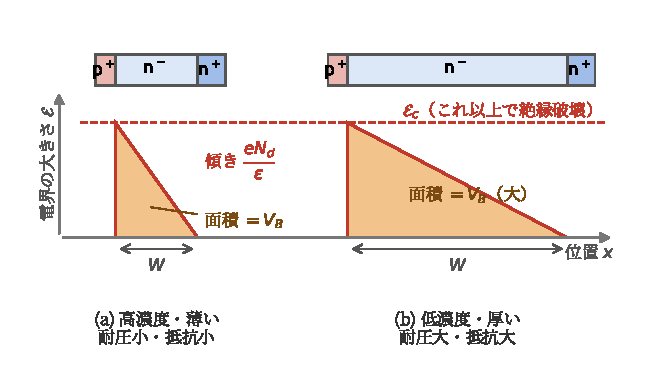
\includegraphics[clip]{figures/fig3.6.eps}
\end{center}
\caption{ドリフト層の電界分布と耐圧。ドナーの固定電荷が一様なので電場は直線的に変わり，接合面で最大の三角形分布になる。電圧はこの三角形の面積で，高さの上限が絶縁破壊電界$\mathcal{E}_c$である。高い耐圧を得るには(b)のように低濃度で厚い層が必要になり，その層がオン状態では抵抗になる}
\label{fig3.6}
\end{figure}

オン状態では，このドリフト層がそのまま直列抵抗になる。
オン抵抗$R_{\mathrm{on}}$とチップ面積$A$の積を\index{とくせいおんていこう@特性オン抵抗}\textbf{特性オン抵抗}$R_{\mathrm{on}}A$といい
（実用上の単位はm$\Omega\cdot$cm$^2$），面積によらない指標である。
導電率$\sigma = e\mu_nN_d$の層の抵抗は$R_{\mathrm{on}} = W/(\sigma A)$だから（2章の例題），$R_{\mathrm{on}}A = W/(e\mu_nN_d)$である。
耐圧を上げると分子の$W$は厚くなり分母の$N_d$は薄くなる ― 薄くも濃くもできないから，$W/N_d$は$V_B$の2乗で効く。
式\ref{eq3.5}と三角形の傾きの条件$N_d = \varepsilon\mathcal{E}_c/(eW)$を使って書き下せば
\begin{equation}
R_{\mathrm{on}}A = \frac{4V_B^2}{\varepsilon\mu_n\mathcal{E}_c^3}
\label{eq3.6}
\end{equation}
を得る。これが本章で最も重要な式である。

\begin{箇条書}
\item $R_{\mathrm{on}}A \propto V_B^2$：\textbf{耐圧を2倍にするとオン抵抗は4倍}になる。この宿命は設計の工夫では消せない
\item 分母は材料定数だけ：$\varepsilon\mu_n\mathcal{E}_c^3$が大きい材料ほど低いオン抵抗で済み，特に$\mathcal{E}_c$は\textbf{3乗}で効く
\end{箇条書}

材料を決めれば，式\ref{eq3.6}は耐圧と特性オン抵抗の平面上に1本の限界線を引く（\FIGref{fig3.7}）。
シリコンの線は\index{しりこんげんかい@シリコン限界}\textbf{シリコン限界}と呼ばれ，
通常の構造のシリコン素子はこの線より下（低抵抗側）へは行けない。
式\ref{eq3.6}はドリフト層だけの下限で，実際にはチャネルやパッケージの抵抗が上乗せされる。

\begin{figure}[ht]
\begin{center}
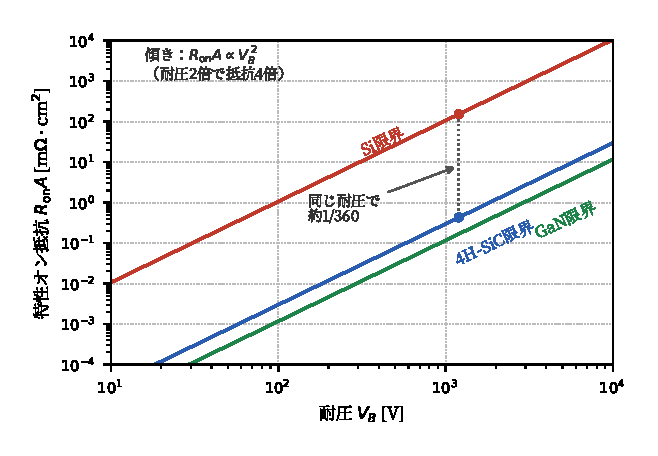
\includegraphics[clip]{figures/fig3.7.eps}
\end{center}
\caption{耐圧と特性オン抵抗のトレードオフ（式\ref{eq3.6}による材料限界線）。$R_{\mathrm{on}}A$は$V_B^2$に比例し（両対数で傾き2），材料の限界線より下へは行けない。SiC・GaNは$\mathcal{E}_c$が約10倍大きいため，限界線が2桁半ほど下にある}
\label{fig3.7}
\end{figure}

\begin{問}
\item バンドギャップ$E_g$が大きい材料ほど絶縁破壊電界$\mathcal{E}_c$が大きくなる理由を，衝突電離の観点から説明せよ。
\end{問}

%%======================================================================
\section{スイッチング損失と高周波化の限界}
\label{sec3.8}

本節では，スイッチが1秒間にオン・オフを繰り返す回数をスイッチング周波数$f$，
1周期のうちオンである時間の割合をデューティ比$D$と呼んで先取りして使う（正式には4章で定義する）。

\subsection{なぜ一瞬で切り替えられないのか}

理想スイッチは一瞬で切り替わるが，実際の素子には準備がいる。
第一に\textbf{容量の充放電}である。
ゲートに反転層を作るには\index{げーとでんか@ゲート電荷}\textbf{ゲート電荷}$Q_g$を出し入れする必要があり，
駆動回路の電流$i_g$では$Q_g/i_g$程度の時間がかかる。
ドレイン側の空乏層に伴う\index{しゅつりょくようりょう@出力容量}\textbf{出力容量}$C_{\mathrm{oss}}$も，電圧が変わるたびに充放電される。
第二に\textbf{少数キャリアの掃き出し}で，ダイオードの逆回復（\ref{sec3.2}節）とIGBTのテール電流（\ref{sec3.5}節）がこれである。
その結果，切り替えには有限の\index{たーんおんじかん@ターンオン時間}\textbf{ターンオン時間}$t_{\mathrm{on}}$と
\index{たーんおふじかん@ターンオフ時間}\textbf{ターンオフ時間}$t_{\mathrm{off}}$がかかる。
MOSFETで数十ns，IGBTでは数百ns〜$\mathrm{\mu}$s級である。

\subsection{切り替えの瞬間に電圧と電流が重なる}

オンでもオフでも消費電力$p = vi$はほぼゼロだが，切り替えの途中では\textbf{電圧と電流が同時にゼロでない}期間が必ずでき，
その間$p = vi > 0$の電力が素子の中で熱になる（\FIGref{fig3.8}）。
インダクタが電流を保とうとする回路（5章以降）では，
ターンオンではまず電圧が$V$のまま電流が$0$から$I$へ立ち上がり，続いて電流が$I$のまま電圧が$V$から0へ下がる。
変化を直線とみなすと瞬時電力の山は底辺$t_{\mathrm{on}}$，高さ$VI$の三角形になり，その面積がターンオン1回の損失である。
ターンオフも同じで，
\begin{equation}
E_{\mathrm{on}} = \frac{1}{2}VIt_{\mathrm{on}},\qquad
E_{\mathrm{off}} = \frac{1}{2}VIt_{\mathrm{off}}
\label{eq3.7}
\end{equation}
となる。
1秒間に$f$回切り替えるときの平均のスイッチング損失電力は
\begin{equation}
P_{\mathrm{sw}} = \frac{1}{2}VI(t_{\mathrm{on}} + t_{\mathrm{off}})f
\label{eq3.8}
\end{equation}
となる。一方，導通損失はデューティ比$D$を使って
\begin{equation}
P_{\mathrm{cond}} = R_{\mathrm{on}}I^2 D
\label{eq3.9}
\end{equation}
であり（IGBTでは$V_{\mathrm{on}}ID$），素子の総損失は
\begin{equation}
P_{\mathrm{total}} = P_{\mathrm{cond}} + P_{\mathrm{sw}}
\label{eq3.10}
\end{equation}
となる。

\begin{figure}[ht]
\begin{center}
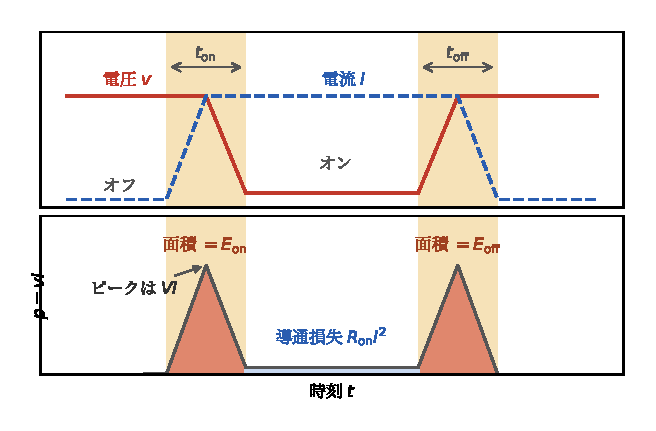
\includegraphics[clip]{figures/fig3.8.eps}
\end{center}
\caption{スイッチング波形と損失。切り替えの途中では電圧と電流が同時に存在し，瞬時電力$p=vi$の山ができる。山の面積が1回あたりのスイッチング損失$E_{\mathrm{on}}$，$E_{\mathrm{off}}$で，山を底辺が切り替え時間$t$，高さが$VI$の三角形とみなせば面積は$\frac{1}{2}VIt$である。オン期間中も小さな導通損失$R_{\mathrm{on}}I^2$が出続ける}
\label{fig3.8}
\end{figure}

\begin{箇条書}
\item $P_{\mathrm{sw}} \propto f$：\textbf{周波数を上げた分だけ損失は正比例で増える}。
導通損失は周波数によらないから，高周波では必ずスイッチング損失が支配的になる
\item $P_{\mathrm{sw}} \propto (t_{\mathrm{on}} + t_{\mathrm{off}})$：
\textbf{切り替えを10倍速くできれば，同じ損失で周波数を10倍にできる}
\end{箇条書}

それでもなぜ高周波化したいのか。
変換回路のインダクタとキャパシタの大きさはおおむね$1/f$で決まり（4章以降），周波数を10倍にできれば装置は10分の1のLとCで済む。
\textbf{小型化と高効率の綱引き}こそ，スイッチング周波数を選ぶという設計行為の正体である。

\begin{例題}[導通損失とスイッチング損失]
\label{rei3.1}
$V = 100$\,V，$I = 10$\,Aを切り替えるMOSFETがある。
$R_{\mathrm{on}} = 50$\,m$\Omega$，$t_{\mathrm{on}} = t_{\mathrm{off}} = 50$\,ns，$D = 0.5$とする。
(a) $f = 100$\,kHzのときの導通損失とスイッチング損失，(b) $f = 1$\,MHzのときのスイッチング損失を求めよ。
\begin{解答}
(a) 式\ref{eq3.9}より$P_{\mathrm{cond}} = 0.05\times10^2\times0.5 = 2.5$\,W。
式\ref{eq3.7}より1回の切り替えの損失は
$E_{\mathrm{on}} + E_{\mathrm{off}} = \frac{1}{2}\times100\times10\times(50+50)\times10^{-9} = 50\,\mathrm{\mu J}$
だから，$f = 100$\,kHzでは$P_{\mathrm{sw}} = 50\times10^{-6}\times10^5 = 5$\,Wと，すでに導通損失を上回る。
(b) $f = 1$\,MHzでは$P_{\mathrm{sw}} = 50$\,Wとなり，導通損失の20倍に達して冷却が追いつかない。
高周波化には切り替え時間そのものを短くするしかない（\ref{sec3.9}節）。
\end{解答}
\end{例題}

係数$1/2$は直線変化の近似で，実務ではデータシートの実測値$E_{\mathrm{on}}$，$E_{\mathrm{off}}$に$f$を掛けて見積もる。
出力容量のエネルギー$\frac{1}{2}C_{\mathrm{oss}}V^2$とゲートの充放電エネルギー$Q_gV_g$も1周期ごとに失われ，やはり周波数に比例する。

%%======================================================================
\section{デバイスの選び方とワイドギャップ半導体}
\label{sec3.9}

\subsection{選択の4軸と各素子の位置づけ}

素子を選ぶ軸は4つである。
\textbf{耐圧}（回路がオフ時にかける電圧に余裕をもって耐えるか，\ref{sec3.7}節），
\textbf{電流と導通損失}（オン特性が抵抗性$R_{\mathrm{on}}I^2$か定電圧性$V_{\mathrm{on}}I$か），
\textbf{速度}（必要な周波数でスイッチング損失を許容できるか，\ref{sec3.8}節），
\textbf{駆動性}（電圧駆動か電流駆動か，\ref{sec3.1}節）である。
本章の5素子をこの軸で整理したのが\TABref{tab3.1}である。
多数キャリアだけで動くMOSFET（\index{ゆにぽーらでばいす@ユニポーラデバイス}\textbf{ユニポーラデバイス}）は速く，
少数キャリアの注入を使うBJT・IGBT・サイリスタ（\index{ばいぽーらでばいす@バイポーラデバイス}\textbf{バイポーラデバイス}）は
高耐圧でも低いオン電圧（IGBTでは\index{ほうわでんあつ@飽和電圧}\textbf{飽和電圧}$V_{\mathrm{CE(sat)}}$と呼ぶ）を保つ代わりに遅く，
多数キャリアだけで整流する\index{しょっときーばりあだいおーど@ショットキーバリアダイオード}\textbf{ショットキーバリアダイオード}（2章）は逆回復がなく高周波の還流に向く。

\begin{table}[ht]
\begin{center}
\caption{本章で学んだ半導体スイッチのまとめと位置づけ。耐圧と周波数は代表的な目安である}
\label{tab3.1}
{\footnotesize
\setlength{\tabcolsep}{3pt}
\begin{tabular}{l|c|c|c|c|c|c}
\hline
素子 & 制御 & 駆動 & オフの制御 & オン特性 & 耐圧 & 周波数 \\
\hline
ダイオード & なし & --- & 電圧の向き & $V_FI$型（〜1\,V） & 〜数kV & 受動 \\
BJT & ベース電流 & 電流 & 可 & $V_{\mathrm{on}}I$型（小） & 〜1\,kV & 〜数十kHz \\
MOSFET & ゲート電圧 & 電圧 & 可 & $R_{\mathrm{on}}I^2$型 & 〜900\,V & 〜MHz級 \\
IGBT & ゲート電圧 & 電圧 & 可 & $V_{\mathrm{on}}I$型（1〜2\,V） & 0.6〜6.5\,kV & 〜20\,kHz \\
サイリスタ & ゲート電流 & 電流 & 不可 & $V_{\mathrm{on}}I$型（1〜2\,V） & 〜10\,kV & 商用周波数 \\
\hline
\end{tabular}
}
\end{center}
\end{table}

MOSFETとIGBTは，導通損失が等しくなる電流$I^* = V_{\mathrm{on}}/R_{\mathrm{on}}$（章末問題\ref{ex3.3}）を境に，
小電流ではMOSFET，大電流ではIGBTが有利になる。
これに周波数の軸を重ねた\FIGref{fig3.9}のすみ分けは，
「伝導度変調は導通損失を減らすがスイッチングを遅くする」という1つのトレードオフの必然である。

\begin{figure}[ht]
\begin{center}
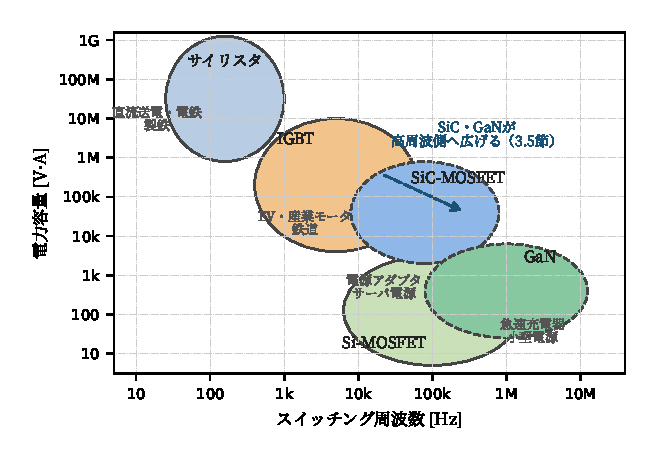
\includegraphics[clip]{figures/fig3.9.eps}
\end{center}
\caption{デバイス選択の地図。スイッチング周波数と電力容量の平面で，各素子は物理の必然としてすみ分ける。SiC・GaNは同じ平面の右上（高周波・大電力側）へ適用範囲を広げつつある}
\label{fig3.9}
\end{figure}

\subsection{損失の行き先 ― 熱抵抗と接合温度}

損失$P_{\mathrm{total}}$はすべて熱になり，チップ（接合部）からパッケージ，放熱器を経て周囲へ逃げていく。
熱の流れにくさを表す量が\index{ねつていこう@熱抵抗}\textbf{熱抵抗}$R_{\mathrm{th}}$（単位K/W）で，
接合部の温度$T_j$は周囲温度$T_a$より
\begin{equation}
T_j = T_a + R_{\mathrm{th}}P_{\mathrm{total}}
\label{eq3.11}
\end{equation}
だけ高くなる。
シリコンの\index{せつごうおんど@接合温度}\textbf{接合温度}の定格は$150\,^{\circ}$C程度である。
たとえば電気自動車用インバータのIGBTで$P_{\mathrm{total}} = 150$\,Wなら，
熱抵抗$0.5$\,K/Wの水冷で温度上昇は$75$\,Kに収まるが，自然空冷（$1$\,K/W以上）では使えない。
\textbf{その損失を何度で捨てるか}まで決めて初めてその素子が使える。

素子は，(1)~\textbf{耐圧}（オフ時の最大電圧が定格電圧の50〜80\,\%に収まるか），
(2)~\textbf{電流}（$I^*$と比べてMOSFETかIGBTか，\ref{fig3.9}），
(3)~\textbf{損失}（周波数$f$を決めて式\ref{eq3.8}〜\ref{eq3.10}），
(4)~\textbf{駆動}（ゲート電荷$Q_g$から駆動回路の規模），
(5)~\textbf{熱}（式\ref{eq3.11}の接合温度が定格内か。収まらなければ冷却か$f$か素子を見直す）の順に選ぶ。
回路が決める耐圧と電流が先，その結果の損失と熱が後である（章末問題\ref{ex3.6}）。

\subsection{なぜワイドギャップ半導体か}

SiCとGaNは，シリコンの約3倍のバンドギャップをもつ
\index{わいどぎゃっぷはんどうたい@ワイドギャップ半導体}\textbf{ワイドギャップ半導体}である（2章，\TABref{tab3.2}）。
注目すべきは絶縁破壊電界$\mathcal{E}_c$の\textbf{約10倍}の差で，これは衝突電離に$E_g$以上のエネルギーが要ること（\ref{sec3.7}節）の必然である。

\begin{table}[ht]
\begin{center}
\caption{Si・4H-SiC・GaNの物性比較（室温の代表値）}
\label{tab3.2}
{\small
\begin{tabular}{l|c|c|c}
\hline
物性 & Si & 4H-SiC & GaN \\
\hline
バンドギャップ $E_g$ [eV] & 1.12 & 3.26 & 3.39 \\
絶縁破壊電界 $\mathcal{E}_c$ [V/m] & $3\times10^7$ & $2.5\times10^8$ & $3.3\times10^8$ \\
電子移動度 $\mu_n$ [cm$^2$/(V$\cdot$s)] & 1350 & 1000 & 1200 \\
比誘電率 $\varepsilon_r$ & 11.7 & 9.7 & 9.0 \\
熱伝導率 [W/(cm$\cdot$K)] & 1.5 & 4.9 & 2.0 \\
\hline
\end{tabular}
}
\end{center}
\end{table}

$\mathcal{E}_c$が10倍になると何が起こるか。\ref{sec3.7}節の式がそのまま答えてくれる。

\begin{箇条書}
\item ドリフト層の厚さ（式\ref{eq3.5}）：$W = 2V_B/\mathcal{E}_c$ → 同じ耐圧を\textbf{10分の1の厚さ}で受け止められる
\item ドーピング濃度：$N_d \propto \mathcal{E}_c^2$ → \textbf{約100倍濃く}できる
\item 特性オン抵抗（式\ref{eq3.6}）：$\mathcal{E}_c^3$に反比例して\textbf{約1000分の1}になる
\end{箇条書}

薄くなった分と濃くなった分が掛け合わさって$\mathcal{E}_c$は3乗で効く
（式\ref{eq3.6}の分母$\varepsilon\mu_n\mathcal{E}_c^3$は\textbf{バリガ性能指数}と呼ばれる）。
移動度と誘電率の差を含めても，限界線は\ref{fig3.7}のとおり2桁半下へ移る。

\begin{例題}[Si MOSFETとSiC MOSFETのオン抵抗比較]
\label{rei3.2}
耐圧$V_B = 1200$\,Vのドリフト層を，シリコンと4H-SiCで設計する。
それぞれの(a)厚さ$W$，(b)特性オン抵抗$R_{\mathrm{on}}A$を求めて比較せよ。
物性値は\ref{tab3.2}を使い，$\varepsilon = \varepsilon_r\varepsilon_0$，$\varepsilon_0 = 8.854\times10^{-12}$\,F/mとする。
\begin{解答}
(a) 式\ref{eq3.5}より，シリコンでは$W = 2\times1200/(3\times10^7) = 80\,\mathrm{\mu m}$，
4H-SiCでは$W = 2\times1200/(2.5\times10^8) = 9.6\,\mathrm{\mu m}$。
(b) シリコンは$\varepsilon = 1.04\times10^{-10}$\,F/m，$\mu_n = 0.135\,\mathrm{m^2/(V\cdot s)}$で，式\ref{eq3.6}より
\begin{eqnarray}
R_{\mathrm{on}}A|_{\mathrm{Si}}
&=& \frac{4\times1200^2}{1.04\times10^{-10}\times0.135\times(3\times10^7)^3} \nonumber\\
&\approx& 1.5\times10^{-5}\,\Omega\cdot\mathrm{m^2} = 152\,\mathrm{m\Omega\cdot cm^2} \nonumber
\end{eqnarray}
4H-SiCは$\varepsilon = 8.6\times10^{-11}$\,F/m，$\mu_n = 0.10\,\mathrm{m^2/(V\cdot s)}$で
\begin{eqnarray}
R_{\mathrm{on}}A|_{\mathrm{SiC}}
&=& \frac{4\times1200^2}{8.6\times10^{-11}\times0.10\times(2.5\times10^8)^3} \nonumber\\
&\approx& 4.3\times10^{-8}\,\Omega\cdot\mathrm{m^2} = 0.43\,\mathrm{m\Omega\cdot cm^2} \nonumber
\end{eqnarray}
同じ耐圧で\textbf{約360分の1}である。
1200\,V級のシリコンではMOSFETをあきらめてIGBTを使うしかなかったが，
SiCはこの領域を\textbf{速いユニポーラデバイスのまま}カバーする。
市販のSiC MOSFETはチャネル抵抗などが加わって理論限界より1けた大きいが，限界線は「そこより先へは行けない」壁である。
\end{解答}
\end{例題}

利点はオン抵抗だけではない。
チップ面積を小さくできるので容量も小さく，同じ損失のままスイッチング周波数を1けた上げられ（式\ref{eq3.8}），
漏れ電流が小さく高温に強く，SiCは熱伝導率もシリコンの約3倍である。
GaNではAlGaN/GaN界面の2次元電子ガスをチャネルに使う横型の\index{へむと@HEMT}\textbf{HEMT}が作れ，MHz級の動作に向く。
現在は650\,V程度まではGaN，1200\,V以上はSiCというすみ分けが進んでいる（\ref{fig3.9}）。

\begin{問}
\item 耐圧1200\,Vのドリフト層をGaNで設計すると，厚さ$W$は何$\mathrm{\mu m}$になるか。
\ref{tab3.2}の値を使い，例題\ref{rei3.2}のシリコンの結果と比較せよ。
\end{問}

これで第I部が完結した。次章からは第II部 ― これらのスイッチにインダクタとキャパシタを組み合わせる電力変換回路の世界に入る。

%%======================================================================
\begin{章末問題}
\item \label{ex3.1}
室温（$kT/e = 0.026$\,V）のダイオードで，順方向電流を10倍にするには順方向電圧をどれだけ増やせばよいか，
式\ref{eq3.2}から求めよ（$\exp(ev_D/kT) \gg 1$としてよい）。

\item \label{ex3.2}
室温（$kT/e = 0.026$\,V）で，同じダイオードに$v_D = +0.5$\,Vをかけたときと$-0.5$\,Vをかけたときの
電流の大きさの比を，式\ref{eq3.2}から概算せよ。

\item \label{ex3.3}
オン抵抗$R_{\mathrm{on}} = 50\,\mathrm{m\Omega}$のMOSFETと，オン電圧$V_{\mathrm{on}} = 1.25$\,V（一定とみなす）のIGBTについて，
電流$I = 10$\,Aと$50$\,Aのときの導通損失をそれぞれ求めて比較せよ。
また，両者の導通損失が等しくなる電流$I^*$を求めよ。

\item \label{ex3.4}
IGBTとサイリスタはどちらもn形とp形を4層に重ねた構造をもつ。
それにもかかわらず，IGBTはゲートでオフできる自己消弧形，サイリスタはオフできない他励形である。
両者の制御のしくみの違い（ゲートがどこにあり，何を動かすか）に着目して，この違いを説明せよ。

\item \label{ex3.5}
電気自動車のインバータで，$V = 400$\,V，$I = 100$\,A，$D = 0.5$の条件でスイッチが動作している。
\begin{enumerate}
\item[(a)] IGBT（$V_{\mathrm{CE(sat)}} = 1.5$\,V，$t_{\mathrm{on}} + t_{\mathrm{off}} = 1\,\mathrm{\mu s}$）を
$f = 10$\,kHzで使うときの導通損失，スイッチング損失，総損失を求めよ。
\item[(b)] (a)のIGBTのまま$f = 50$\,kHzに上げると総損失はいくらになるか。
\item[(c)] SiC MOSFET（$R_{\mathrm{on}} = 10$\,m$\Omega$，$t_{\mathrm{on}} + t_{\mathrm{off}} = 100$\,ns）を
$f = 50$\,kHzで使うときの総損失を求め，(b)と比較せよ。
\end{enumerate}

\item \label{ex3.6}
次の3つの用途それぞれについて，\ref{sec3.9}節の素子を選ぶ手順に従い，
\ref{tab3.1}と\ref{fig3.9}を参考に適切なスイッチング素子を選び，耐圧・電流・周波数・駆動性の4軸から理由を述べよ。
\begin{enumerate}
\item[(a)] ノートPC用ACアダプタ（入力AC100\,V，出力65\,W，数百kHz動作）
\item[(b)] 電気自動車の駆動用インバータ（電池800\,V，最大出力150\,kW）
\item[(c)] 直流送電の変換所（数百kV・GW級，商用周波数）
\end{enumerate}
\end{章末問題}
